\section{System Implementation}
% Flutter state management spostato più in alto essendo backend posso dire
\subsection{Firebase}
\subsubsection{Firebase Authentication}
\label{subsubsec:firebaseAuthentication}
Setting up the Authentication was pretty straightforward, as also previously explained (see \cref{subsubsec:authenticationService}). All it took was going to the firebase console in the project settings and register both the mobile application and the web one. After that, in the authentication tab the desired Sign-in providers have been enabled (in our case email/password and Google). The firebase platform and the underlying google structure handled the rest by generating both the API keys to access the firebase services and the OAuth 2.0 clients to authenticate the users.

% \begin{figure*}
%     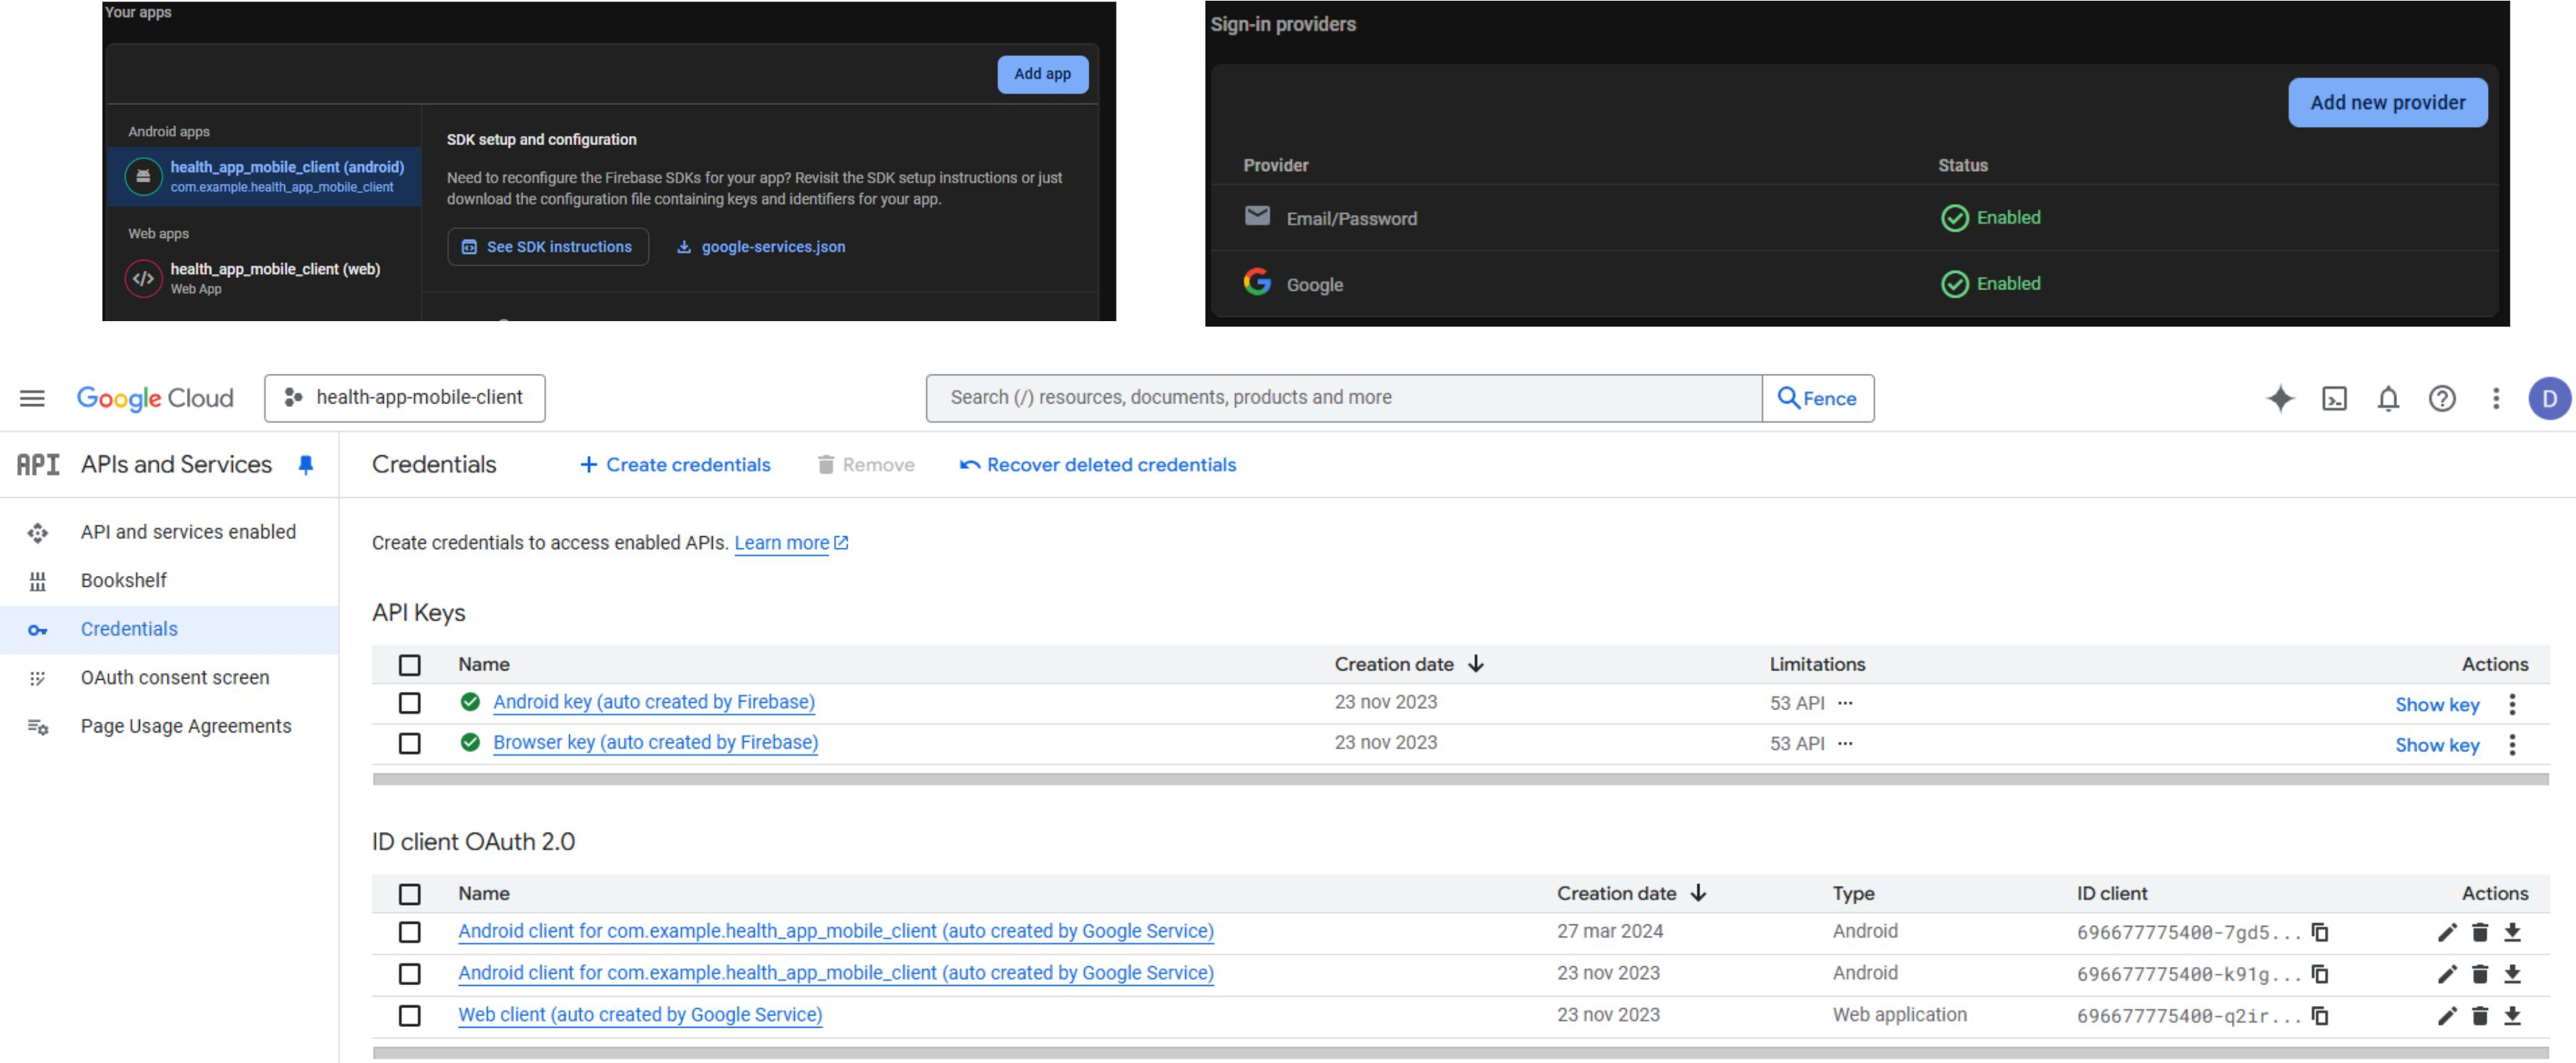
\includegraphics[width=1.0\linewidth]{./images/authentication.jpg}
%     \caption{Registered apps and sign-in providers in the firebase console and generated api keys and OAuth 2.0 clients in the cloud console.}
% \end{figure*}

\noindent In case of the email/password authentication approach, also email templates have been employed:
\begin{itemize}[nosep] % 'nosep' removes extra spacing between items
    \item \textbf{Email address verification:} once a user signs up, a confirmation email is sent to verify his registered email address.
    \item \textbf{Password reset:} in case a user forgets his password, he can request a password reset email.
    \item \textbf{Email address change:} in case a user change his email address, a confirmation email is sent to the original address, so that the user can review the change.
\end{itemize}

\noindent At this point for the \textbf{mobile client} side the firebase dependencies (in particular firebase\_ui\_auth and firebase\_ui\_oauth\_google) have been employed to perform the authentication and the sign-in process. The already well made components already provide the possibility to sign-in or eventually register in case the user is not already registered, as well as manage the user profile once logged in. They are also highly customizable, allowing us to change the UI to match the app's theme. As additional logic, only the authentication state had to be handled in order to redirect the user to the home page once the authentication is successful. This has been done through a \texttt{StreamBuilder} widget and by using \texttt{FirebaseAuth.instance.authStateChanges()}, that notifies about the user's sign-in state as the source stream. In this way, any change is listened and if the user signs in or out the interface is updated coherently.
\newpage
\noindent About the \textbf{web application client} instead, no already-made components were available, so the profile management screen like the mobile one has not been implemented, since it is an admin interface. The react \texttt{createContext} and \texttt{useContext} hooks have been employed to handle the authentication state: it was done by using a context in the react application and providing it at the root level so that the whole application could access the authentication state. This state is updated after performing authentication operations and the components that depend on it are updated accordingly, allowing to display the correct screens once authentication is performed.   

\begin{figure*}
    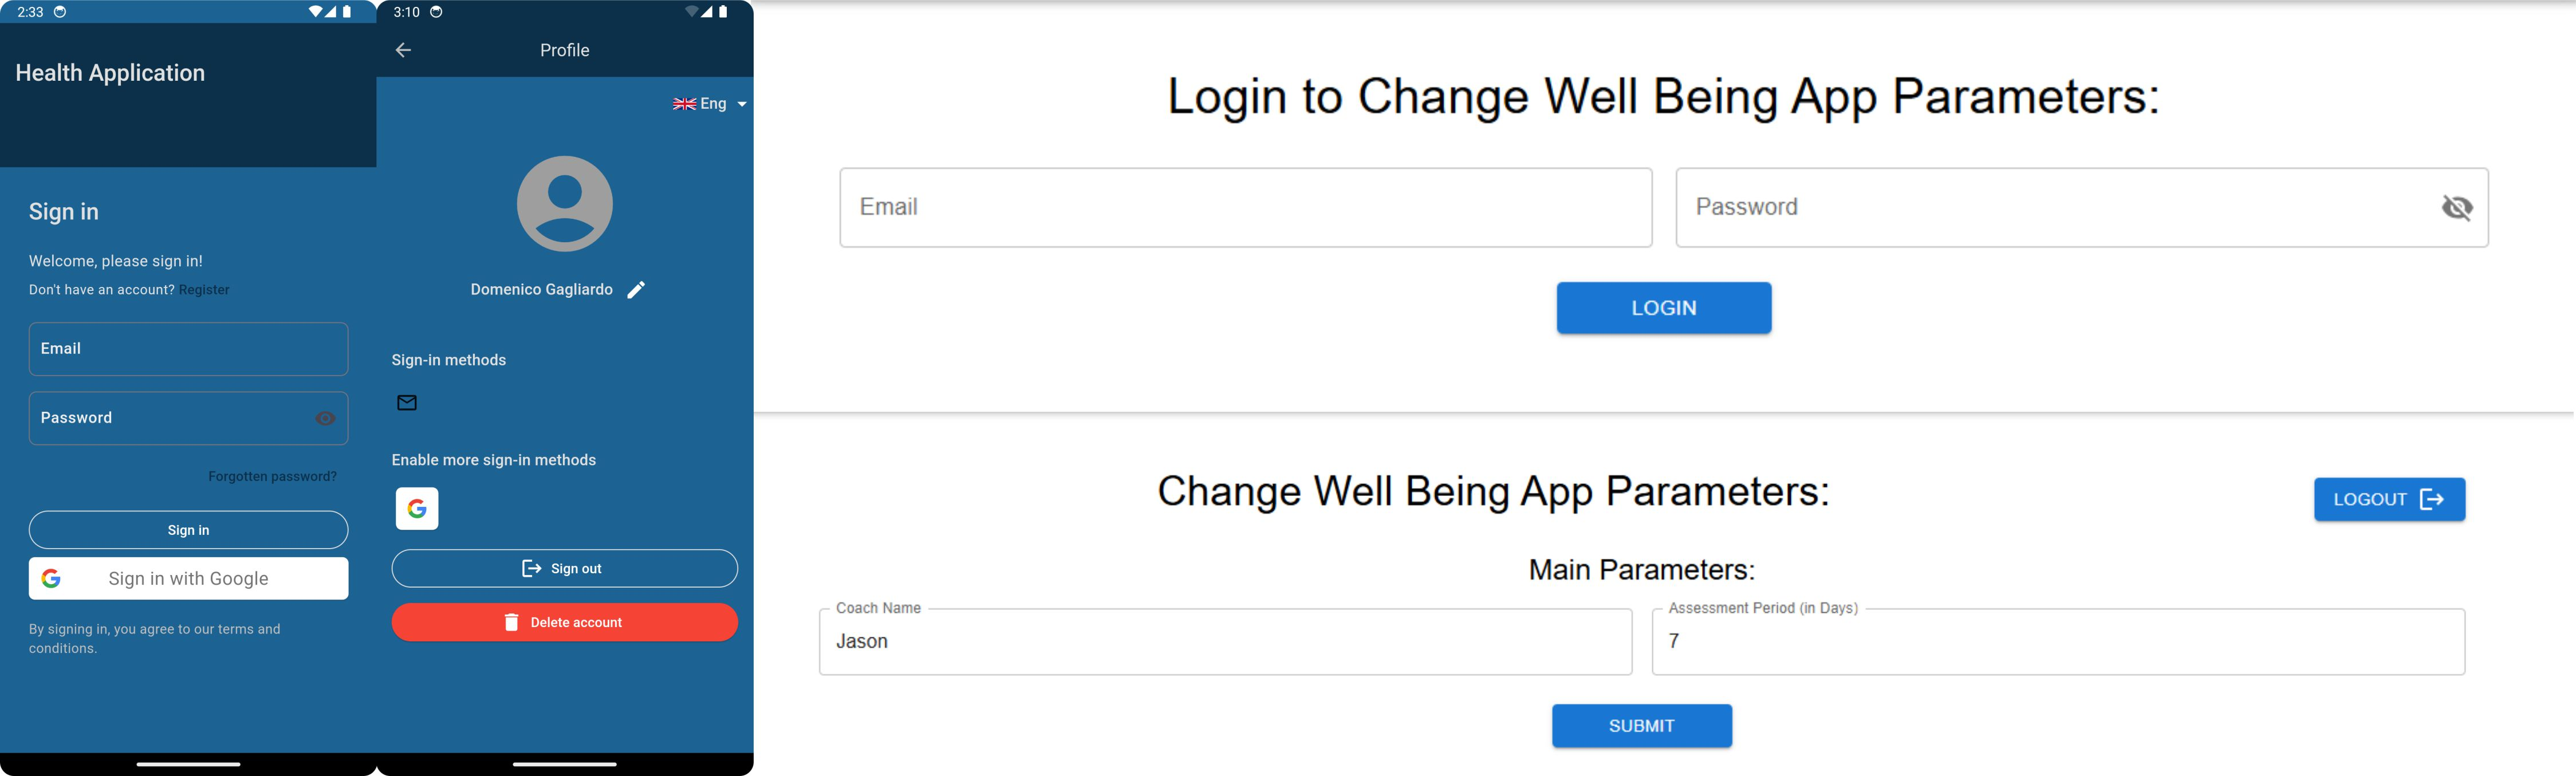
\includegraphics[width=1.0\linewidth]{./images/authenticationScreens.jpg}
    \caption{Authentication Screens of the mobile client (sign in and profile management) on the left and web client on the right.}
\end{figure*}

\subsubsection{Cloud Firestore Database}
Taking into account the data-related requirements (see \cref{tab:fr3}), the database has been implemented accordingly by storing all the data in the most efficient way possible. \newline The database structure is as follows:

\begin{itemize}[nosep] % 'nosep' removes extra spacing between items
    \item The \textbf{users} collection, used to manage main users informations, with each document having the following fields:
    \label{subsubsec:usersCollection}
    \begin{itemize}[nosep]
        \item The \texttt{UID} field, that uniquely identifies the user.
        \item The \texttt{goals} field (composed of \texttt{calories}, \texttt{sleep} and \texttt{steps} as inner fields) that represents the user's goals.
        \item The \texttt{language} field, that represents the app language set and preferred by the user.
        % wearable non in metrics ma scrivo così che fà cacare senò
        \item The \texttt{metrics} field (composed of \texttt{birthDate, height, nickname, sex, waist circumference, weight} and \texttt{wearable} as inner fields) that represents the user's personal information.
    \end{itemize}
\end{itemize}

\begin{itemize}[nosep] % 'nosep' removes extra spacing between items
    \item The \textbf{user\_data} collection, used to manage additional users informations, with each document having the following fields:
    \begin{itemize}[nosep]
        \item The \texttt{userId} field, that links those data with the corresponding user.
        \item The \texttt{current\_notification} field that used in combination with the \newline \texttt{notification\_counter} field allows to implement the notification logic (see \cref{subsec:notifications} for more details).
        \item The \texttt{lastBackupDate} field, that saves the last time that the user performed a backup of his data.
        \item The \texttt{weightData} array field that stores the user's weight information, implementing an history of this metric, alsop present in the \texttt{users} collection for each user. Each element of the array has the \texttt{date} and \texttt{weight} fields.    
        \item The \texttt{waistCircumferenceData} array field that stores the user's waist circumference information, implementing an history of this metric, alsop present in the \texttt{users} collection for each user. Each element of the array has the \texttt{date} and \texttt{waist} \newline \texttt{circumference} fields.
        % qui anche userId ma inutile perchè già in user_data non lo scrivo
        \item The \texttt{emotionalData} array field that stores the user's emotional information. Each element of the array has the \texttt{date}, \texttt{negative} and \texttt{positive} fields.
        \item The \texttt{bodyTestBalanceData} array field that stores the user's body balance information. Each element of the array has the \texttt{date}, \texttt{leftLeg}, \texttt{rightLeg} and \texttt{tandemWalk} fields.
        \item The \texttt{bodyTestStrengthData} array field that stores the user's body strength information. Each element of the array has the \texttt{date}, \texttt{absCount}, \texttt{gripTest}, \texttt{pushUpCount} and \texttt{squatCount} fields.
        \item The \texttt{completedLessons} array field that stores the user's completed lessons information. Each element of the array has the \texttt{lessonId} to which it refers to and a \texttt{completedPills} boolean array field used to store how many pills of the lesson have been read (true) or not (false).
        \item The \texttt{completedQuizzes} array field that stores the user's completed quizzes information. Each element of the array is the \texttt{quizId}: if present means that user has completed that quiz.
    \end{itemize}
\end{itemize}
\newpage
\begin{itemize}[nosep] % 'nosep' removes extra spacing between items
    \item The \textbf{foodRecords} collection, used to manage the food informations for the users, with each document having the following fields:
    \begin{itemize}[nosep]
        \item The \texttt{userID} field, that links those data with the corresponding user.
        \item The \texttt{date} field, storing the food entry recording date.
        \item The \texttt{foodGroup} field, that identifies the type of food (like water, vegetables and so on).
        \item The \texttt{amount} field, that represents the food quantity (e.g. 250 ml if a liquid food or 250 gr if a solid food).
    \end{itemize}
\end{itemize}

\begin{itemize}[nosep] % 'nosep' removes extra spacing between items
    \item The \textbf{lessons} collection, used to manage the available lessons for the users, with each document having the following fields:
    \begin{itemize}[nosep]
        \item The \texttt{id} field, that uniquely identifies the lesson.
        \item The \texttt{quizId} field, that links the quiz related to that lesson.
        \item The \texttt{title} field, that represents the lesson title.
        \item The \texttt{titleIta} field, that represents the italian lesson title.
        \item The \texttt{pills} array field, that represents the list of pills that the lesson is made up of, where each element is a single pill.
        \item The \texttt{pillsIta} array field, that essentially is the italian version of the above \texttt{pills} field.
    \end{itemize}
\end{itemize}

\begin{itemize}[nosep] % 'nosep' removes extra spacing between items
    \item The \textbf{quizzes} collection, used to manage the available quizzes for the users, with each document having the following fields:
    \begin{itemize}[nosep]
        \item The \texttt{id} field, that uniquely identifies the quiz.
        \item The \texttt{questions} array field, that represents the questions of that quiz. Each questions has the \texttt{questionText}, \texttt{correctAnswer} fields and \texttt{possibleAnswers} array field, that respectively represents the question, the correct answer and the list of possible answers, where each element is an answer.
        \item The \texttt{questionsIta} array field, that essentially is the italian version of the above \texttt{questions} field.
    \end{itemize}
\end{itemize}
\newpage
\begin{itemize}[nosep] % 'nosep' removes extra spacing between items
    \item The \textbf{notifications\_text} collection, used to manage the mobile application parameters displayed for the users and editable by the admin through the web application. It is composed of 3 documents:
    \begin{itemize}[nosep]
        \item The first document, that contains two fields called \texttt{coach\_name} and \newline \texttt{assessment\_period} that represents the name of the app assistant and the length of the assessment perios (in days) used for the notification cycle (see \cref{subsec:notifications} for more details).
        \item The second document, that contains several strings fields used to customize the onBoarding experience of the user as well as the data insertion operations. we have up to three fields for the onBoarding (\texttt{onBoarding1,onBoarding2,onBoarding3}), 7 fields for the body test balance data insertion (\texttt{body\_test\_balance1} up to 7), 6 fields for the body test strength data insertion (\texttt{body\_test\_strength1} up to 6), one field for the emotional data insertion (\texttt{emotional\_life\_test}), one field for the assessment (\texttt{assessment}) and one field for the food insertion (\texttt{daily\_reminder\_food}).
        \item The third document, that similarly to what has been done with the lessons and quizzes, contains the italian version of the second document.
    \end{itemize}
\end{itemize}

\subsection{User OnBoarding and Registration}
As explained before (see \cref{subsubsec:firebaseAuthentication}), the user registration and sign-in process is mainly managed by the firebase authentication service. However, some additional initialization steps are required, in order to setup all the documents needed in the database collections for the user, once is registered for the first time. When the user registers for the first time and it interact with ui authentication components of firebase, instead of displaying the main page of the application, the user is redirected to the onBoarding page. Here essentially almost all the information needed to initialize the user document inside the users collection (see \cref{subsubsec:usersCollection}) are asked to be inserted. The proper validation is enforced in case of input errors, preventing the user from proceeding and when the user inserted all the data, all the needed documents and fields for that user are created and the home page is displayed. 
\clearpage
\begin{figure*}
    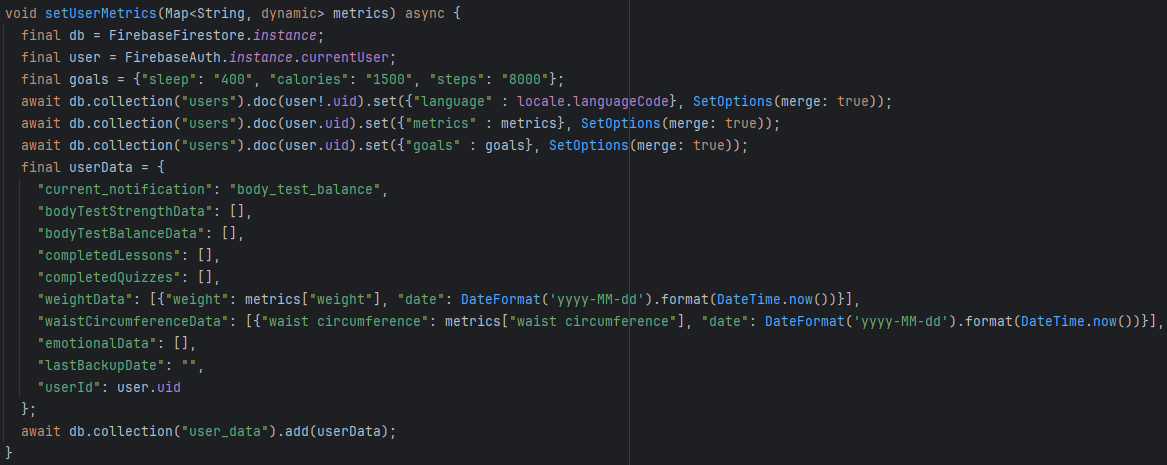
\includegraphics[width=1.0\linewidth]{./images/onBoarding.png}
    \caption{Function Called at the end of the onBoarding process to setup all the needed documents/fields for the user.}
\end{figure*}

\noindent Only the goals are not asked to be inserted in the onBoarding process to avoid make it too long and boring. They have a default value and can be edited in the personal information page at any time.
\subsection{Health Data Backup with Cloud Storage}
In order to perform the backup of the health data and satisfy the related requirement (see \cref{tab:fr3}), the cloud storage service has been employed. The main reason lies behind the fact that health data can be pretty large, so using the Cloud Firestore Database to store them would be inefficient and expensive. For this reason the health data are stored on the cloud storage into JSON files, one for each backup. The backup task is performed thanks to the workmanager library by running a background task in background, allowing to execute the backup even if the app is not opened or actively used in that moment. However, since these tasks run on a separate background isolate, retrieving the health data directly there is not possible, since it was not possible to retrieve the permission.
\newpage For this reason, the backup implementation is structured into three phases:
\begin{enumerate}[nosep] % 'nosep' removes extra spacing between items
    \item In the first phase, that takes place at each application startup, the \newline \texttt{performLocalBackup} function is called. This function retrieves the health data from the database (starting from the lastBackupDate field taken from the user\_data collection for each user) and stores them into a JSON file in the local storage of the device, named with \texttt{Datetime.now().toIso8601String()} to guarantee univocity. After that the lastBackupDate field is coherently updated to \texttt{Datetime.now()}. This local backup is performed with a daily frequency, so if the app is opened more than once a day or simply no data are available the function returns immediately, to avoid to increase the frequency or to create an empty file.
    \item In the second phase, that takes place immediately after the first one, the workmanager background task is scheduled through the \texttt{scheduleBackupTask} function. Is scheduled as a periodic task with the same frequency of the local backup (daily). Also in this case, if the app is opened more than once a day, even if the function is called multiple times, the task id guarantees that the task still is scheduled once.
    \item In the third phase, that takes place when the workmanager background task triggers and is executed, Firebase is initialized in the background isolate and the \texttt{performStorageBackup} function is called. This function loops through the JSON files saved in the local storage of the device and it uploads them to the storage. In case of successful upload, these files are marked for deletion and a second loop proceeds to delete them from the local storage of the phone. In case of failure, the files are not deleted and they will be uploaded when the task is triggerring again. These files are saved in a folder named with the user UID to guarantee univocity and to avoid conflicts between different users' backups, while the filename is also unique, since it is the same that was defined in the \texttt{performLocalBackup} function.
\end{enumerate}

\begin{figure*}
    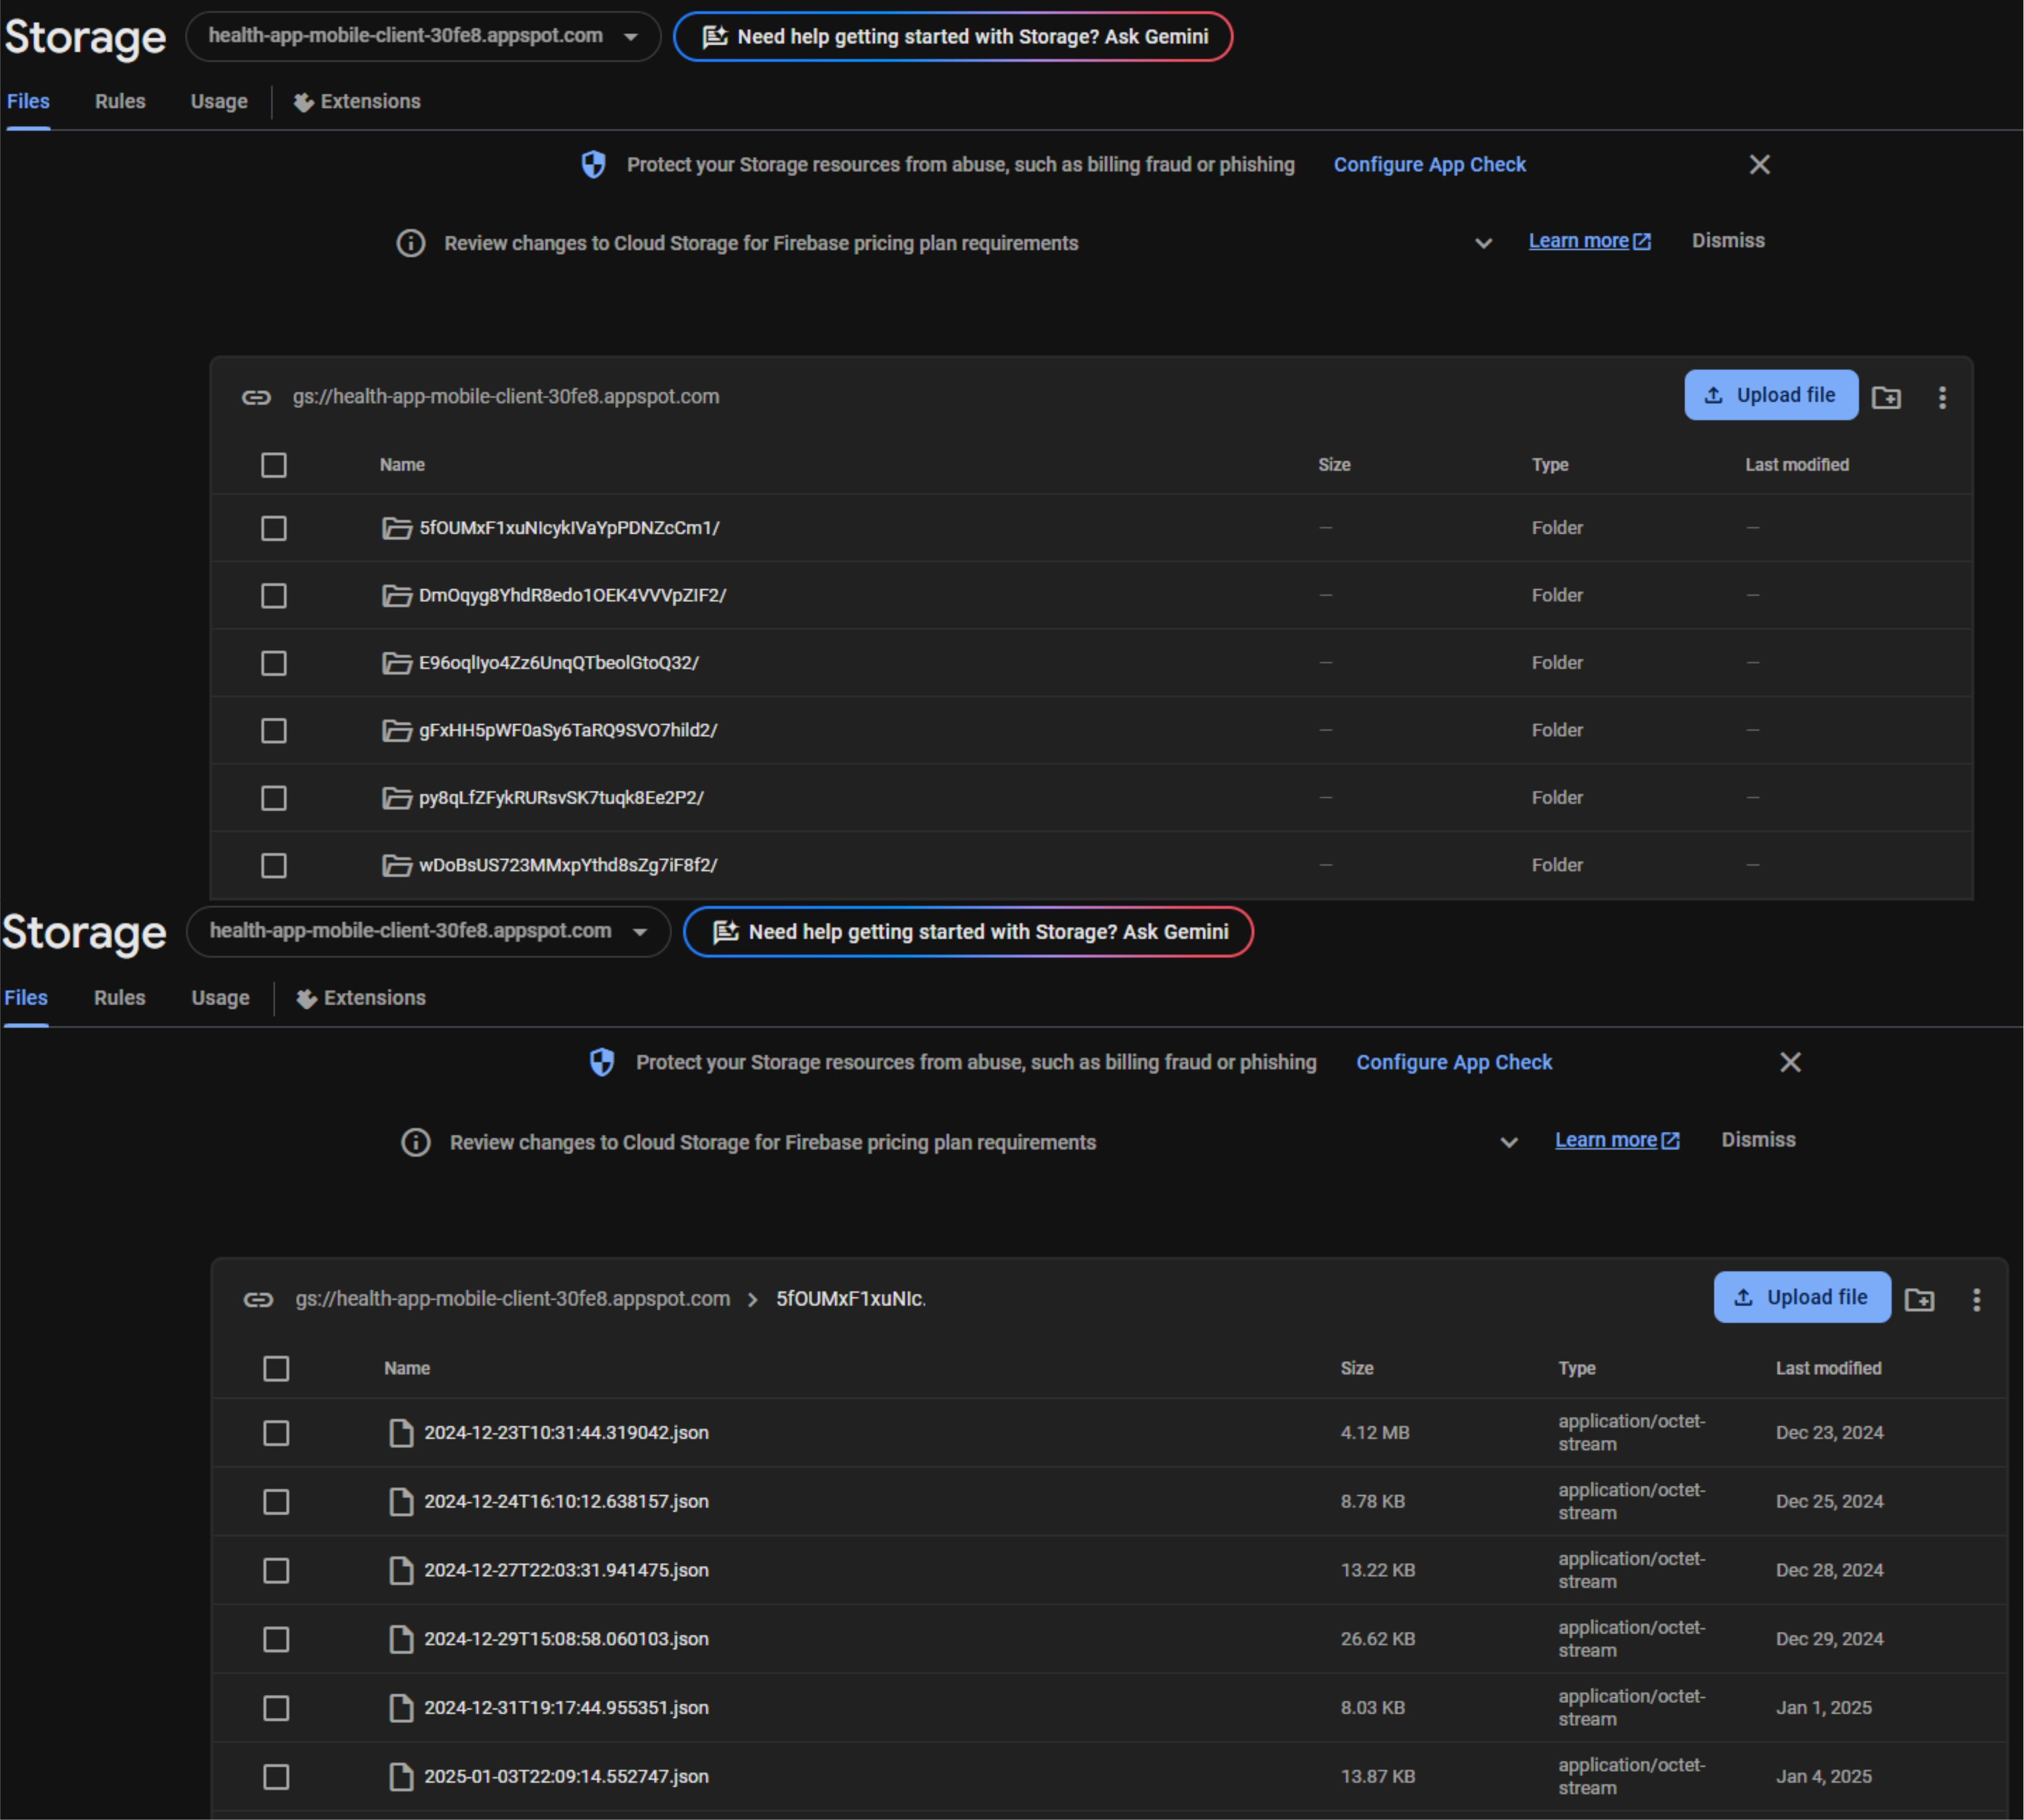
\includegraphics[width=1.0\linewidth]{./images/backup.jpg}
    \caption{Cloud Storage view of the users folder and a single user folder containing the JSON files of the backup.}
\end{figure*}
% \noindent Even if the lastBackupDate field is updated in the first pahse and the actual storage backup happens in the third phase,  
\subsection{Database Data Visualization}
\subsubsection{Home Page}
\subsubsection{Health Measures}
\subsubsection{Personal Information}

\subsection{Database Data Insertion}
\subsubsection{Home Page}
\subsubsection{Health Measures}
\subsubsection{Personal Information}

\subsection{Health Data Visualization}
anche goal firebase con soglia massima
\subsubsection{Home Page}
\subsubsection{Health Measures}

\subsection{Lessons and Quiz}
\subsubsection{Lessons and Quiz Parameters Editing}
frontend

\subsection{Notifications}
\label{subsec:notifications}

implementation e firebase current\_notification e notification \_counter
\subsubsection{Notification Parameters Editing}
frontend 

\subsection{MultiLanguage}
implementation e firebase language field
(collezioni duplicate per multi lingua, gestione dei parametri sempre in collezione a parte) + definizione classe file traduzione etc.
